\setauthorname{Lukas Schachinger}

\chapter{User Interface (UI) und Interaktion}

\begin{quote}
\emph{\glqq Im Interface begegnet der Spieler dem Spiel. [...] Die Schnittstelle zwischen Mensch und Computer/Konsole etc.\grqq}~\cite[][Game Design und Produktion: Grundlagen, Anwendungen und Beispiele; p.~161]{GameDesign} \\ 
\end{quote}

Das \bettergls{UI}{1} im Spieldesign ist fast der wichtigste Teil der Spielentwicklung, wenn man das Design des eigentlichen Spieles außen vornimmt. Ohne eine gute Menüführung und ein gut entworfenes User Interface ist es schwer, dass Spielerinnen und Spieler das Spiel verstehen und spielen können. 

\begin{figure}[H]
  \centering
  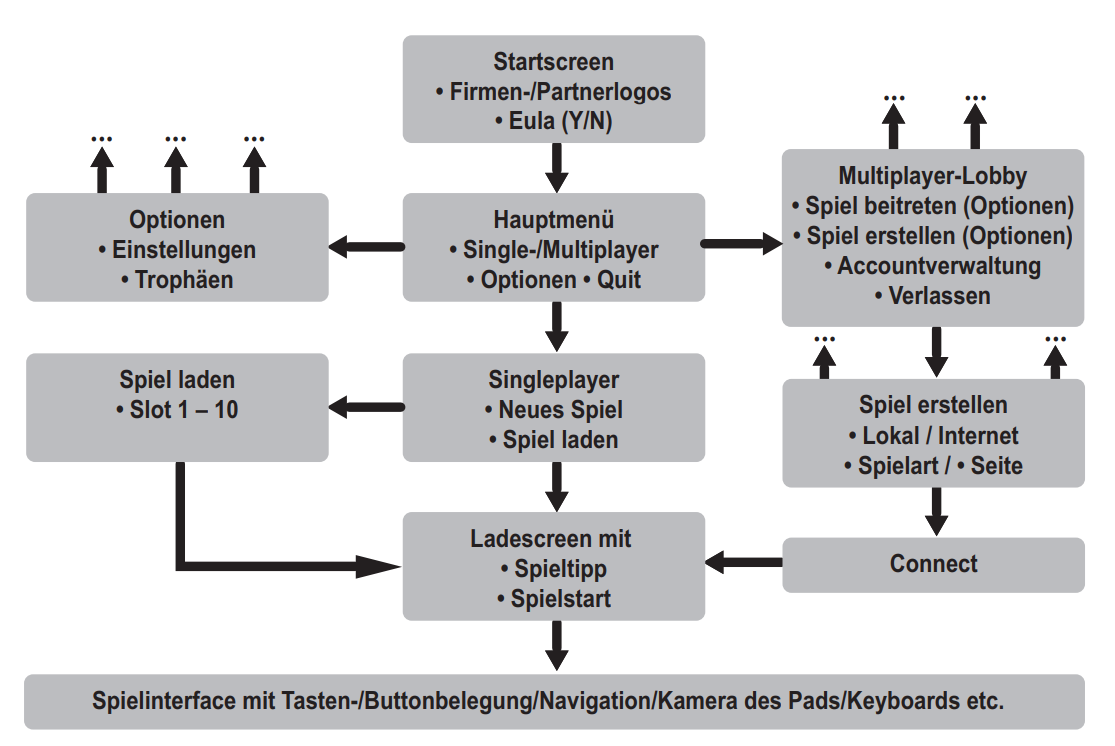
\includegraphics[width=0.6\textwidth]{chapters/03/images/Spielinterface.png}
  \caption{Ein Beispiel eines Dialogbaumes von einem Computerspiel.}
  \label{htl01}
\end{figure}

Der abgebildete Dialogbaum zeigt die verschiedenen Menüs und Screens die ein Computerspiel haben kann. Diese unterscheiden sich in den unterschiedlichen Arten von Spielen. Bei einem \bettergls{multiplayer}{2}-Spiel soll die Möglichkeit geboten werden, ein Spiel zu erstellen oder einem beizutreten. Während es bei einem \bettergls{singleplayer}{3} wichtig ist, Spielstände speichern und laden zu können.

\pagebreak

Das User Interface des Prototyps unterteilt sich in drei verschiedene Aspekte:

\begin{itemize}
    \item Hauptmenü
    \item User Interface während des Spieles
    \item Pausemenü
\end{itemize}

\noindent
Bei der Entscheidung, welche Komplexität das User Interface des Prototyps haben soll, fiel die Wahl auf ein simples Design. 
Das User Interface soll einerseits die Schlichtheit des eigentlichen Spieles wiederspiegeln und andererseits alle für das Spiel wichtigen Informationen darstellen.

\section{Gestaltung des Hauptmenüs}

Im Folgenden wird das Gestalten der Benutzeroberfläche für das Hauptmenü erläutert. 
Das Hauptmenü in der Spielentwicklung ist vergleichbar mit einem Türvorleger vor einer Haustür. Es soll das Willkommenschild für das eigentliche Spiel sein. 
Mithilfe dieses ersten Eindrucks ist es möglich zu erkennen, um welche Art von Spiel es sich handelt. Das \bettergls{theme}{1} des Spieles spiegelt sich in dem Design des Hintergrundes und in der Schriftart des Hauptmenüs wieder. Die Komplexität steht bei vielen Spielen in direkter Korrelation mit der Anzahl an Einstellungen in dem Hauptmenü.

\pagebreak

\subsection{Das Hauptmenü des Prototyps}

Das Hauptmenü des Prototyps besteht aus mehreren Komponenten. Die Hauptkomponente ist ein \bettergls{canvas}{1}. Diesem untergeordnet ist ein Bild, ein \bettergls{gameObject}{2} für das Hauptmenü und ein Game-Objekt für das Optionsmenü. Diese beiden Spiel-Objekte sind die eigentlichen Menüs, die dementsprechen ein- und ausgeblendet werden. Die Knöpfe, die der User betätigen kann, sind den Game-Objek<ten für das Hauptmenü und dem Optionsmenü untergeordnet. 

\subsubsection{Der Hintergrund}
Der Hintergrund des Hauptmenüs ist ein PNG von der \bettergls{skybox}{3} des Spiels. 
\subsubsection{Die Buttons}
Die Abbildungen \ref{htl02a} und \ref{htl02b} zeigen das Hauptmenü (links) und das Optionsmenü (rechts) des Prototyps. In dem Hauptmenü gibt es drei verschiedene Buttons: Play, Options and Quit. Play startet den Spielablauf, Options öffnet das Optionsmenü und Quit schließt das Spiel. In dem Optionsmenü befindet sich die Lautstärkenregelung. Der \glqq Back\grqq \space Button dient dazu zurück in das Hauptmenü zu kommen, befindet sich an letzter Stelle des Optionsmenüs.

\begin{figure}[H]
    \centering
    \begin{minipage}{0.4\textwidth}
        \centering
        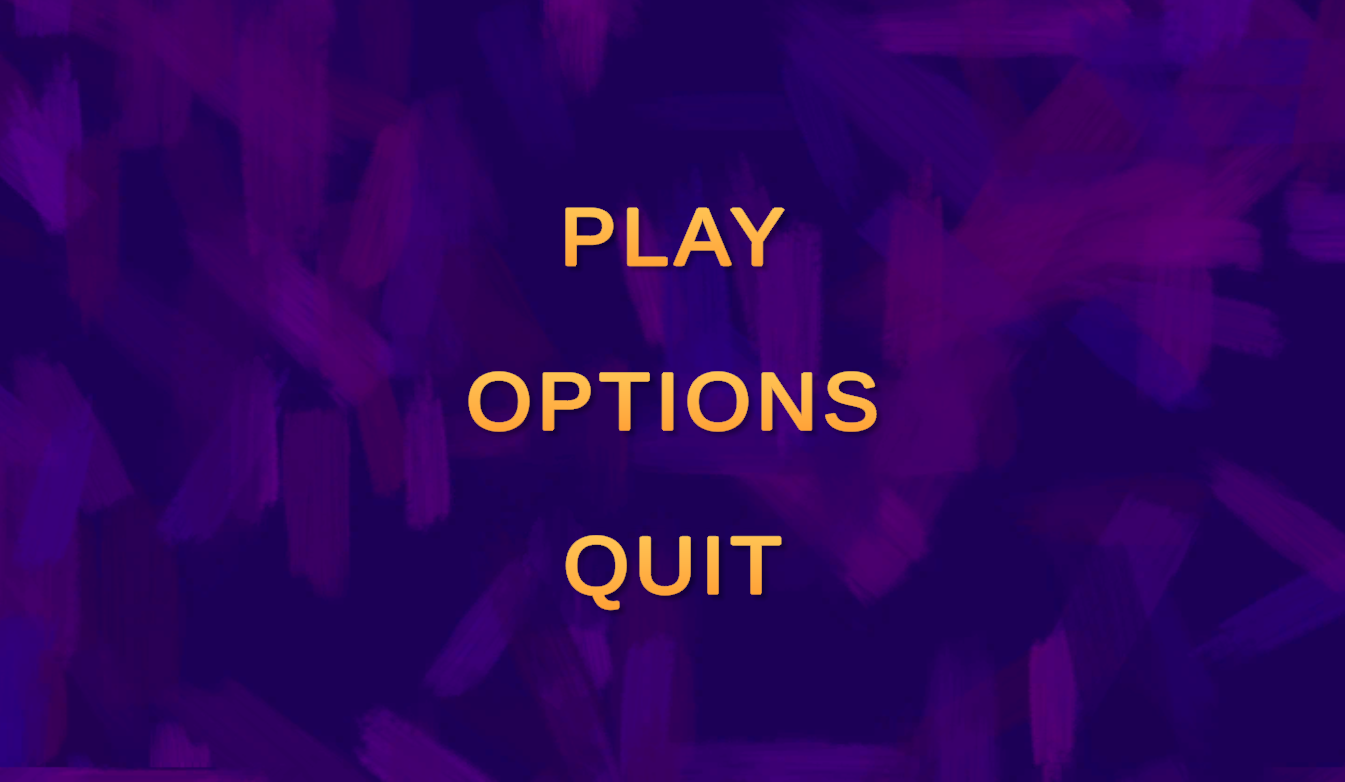
\includegraphics[width=\linewidth]{chapters/03/images/MainMenu.png}
        \caption{Das Hauptmenü des Prototyps.}
        \label{htl02a}
    \end{minipage}%
    \hspace{1cm}% Adjust the space here as needed
    \begin{minipage}{0.4\textwidth}
        \centering
        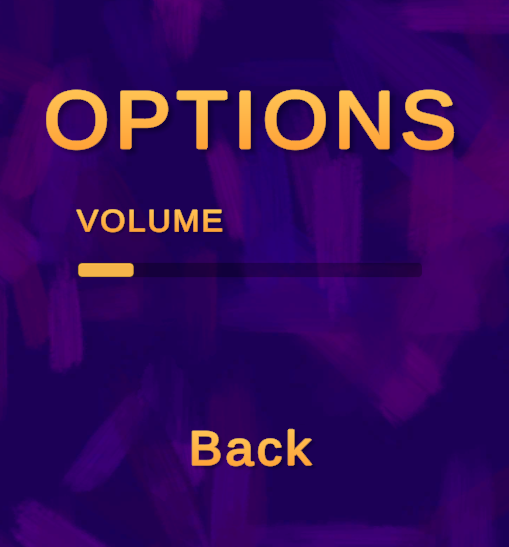
\includegraphics[width=\linewidth]{chapters/03/images/OptionsMainMenu.png}
        \caption{Das Optionsmenü des Prototyps.}
        \label{htl02b}
    \end{minipage}
\end{figure}

\section{Code behind des Menüs}

Der \bettergls{code-behind}{1} des Menüs ist sehr simpel gehalten und auch einfach zu verstehen.

% C#
\begin{lstlisting}[language=CSharp,caption={Main Menu Klasse.},label=code:mainmenu]
public class MainMenu : MonoBehaviour
{
    public void PlayGame()
    {
        var activeScene = SceneManager.GetActiveScene();
        SceneManager.LoadScene(activeScene.buildIndex + 1);
    }

    public void QuitGame()
    {
        Debug.Log("Quit");
        Application.Quit();
    }
}
\end{lstlisting}
Der SceneManager ist ein einfacher Weg mittels einer Art von \bettergls{statemachine}{2} eine Menüführung aufzubauen. In der nächsten Abbildung wird die Build-Reihenfolge der Scenes dargestellt.

\begin{center}
    \begin{figure}[h]
        \centering
        \includegraphics*[width=1\textwidth]{chapters/03/images/SceneManager.png}
        \caption{Der SceneManager in den Build Settings.}
        \label{htl04}
    \end{figure}
\end{center}

\noindent
Mittels der Code Zeile: 
% C#
\begin{lstlisting}[language=CSharp]
    SceneManager.LoadScene(activeScene.buildIndex + 1);
\end{lstlisting}
kann von der Menü Scene, die an der Stelle 0 ist zu der Projekt Scene, die an der Stelle 1 ist, gewechselt werden.

\pagebreak

\subsection{Die Funktion dem Button zuordnen}

In der nächsten Abbildung ist ein Ausschnitt der Properties des Play Buttons zu sehen. Bei der \verb+On Click ()+ Property wurde das \verb+MainMenu+ Skript hinzugefügt. Nachdem das Skript dort ausgewählt wurde, ist es möglich Methoden von diesem als Aktion für den Button auszuwählen. 

\begin{figure}[H]
    \centering
    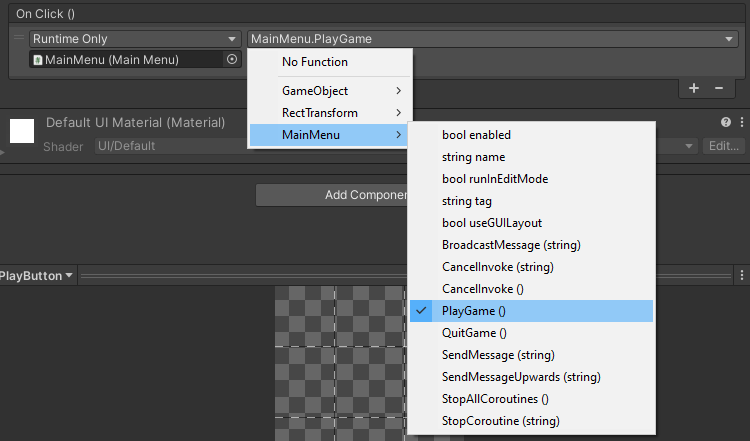
\includegraphics[width=0.6\textwidth]{chapters/03/images/PlayButton.png}
    \caption{Abbildung der Properties des Play Buttons.}
    \label{htl05}
\end{figure}

\section{Pausemenü und Game Over Screen}


Die Pause-Funktion ist ein wichtiger Teil eines Spiels, da sie den Spielern die Möglichkeit bietet, das Spiel zu pausieren, Einstellungen anzupassen oder sogar das Spiel zu verlassen, ohne den Fortschritt zu verlieren. Ebenso bedeutend ist der Game Over Screen, der dem Spieler nach einem Scheitern die Möglichkeit gibt, das Spiel neu zu starten oder komplett zu beenden.

\begin{figure}[H]
    \centering
    \begin{minipage}{0.4\textwidth}
        \centering
        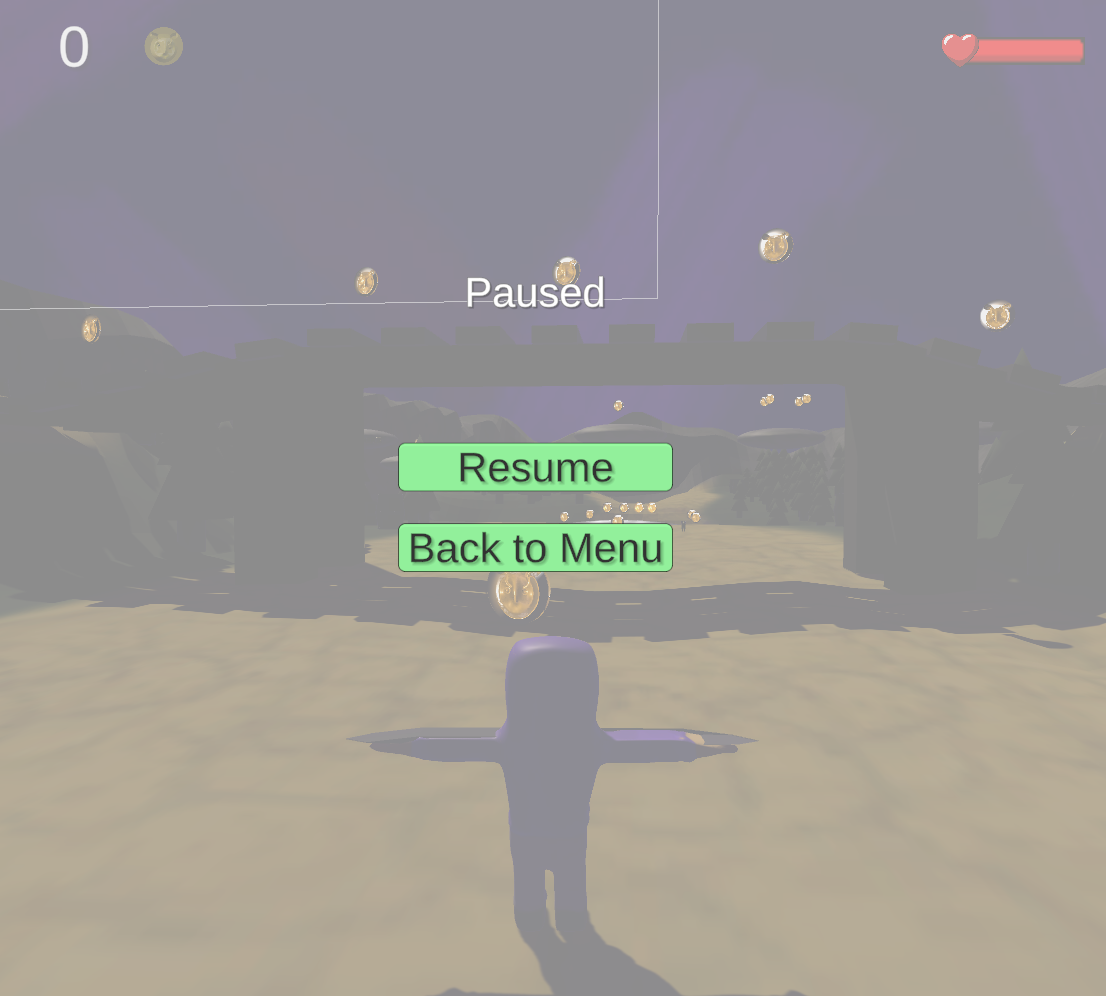
\includegraphics[width=\linewidth]{chapters/03/images/GamePaused.png}
        \caption{Das Game Paused UI des Prototypen.}
        \label{UI01}
    \end{minipage}
    \hspace{1cm}
    \begin{minipage}{0.4\textwidth}
        \centering
        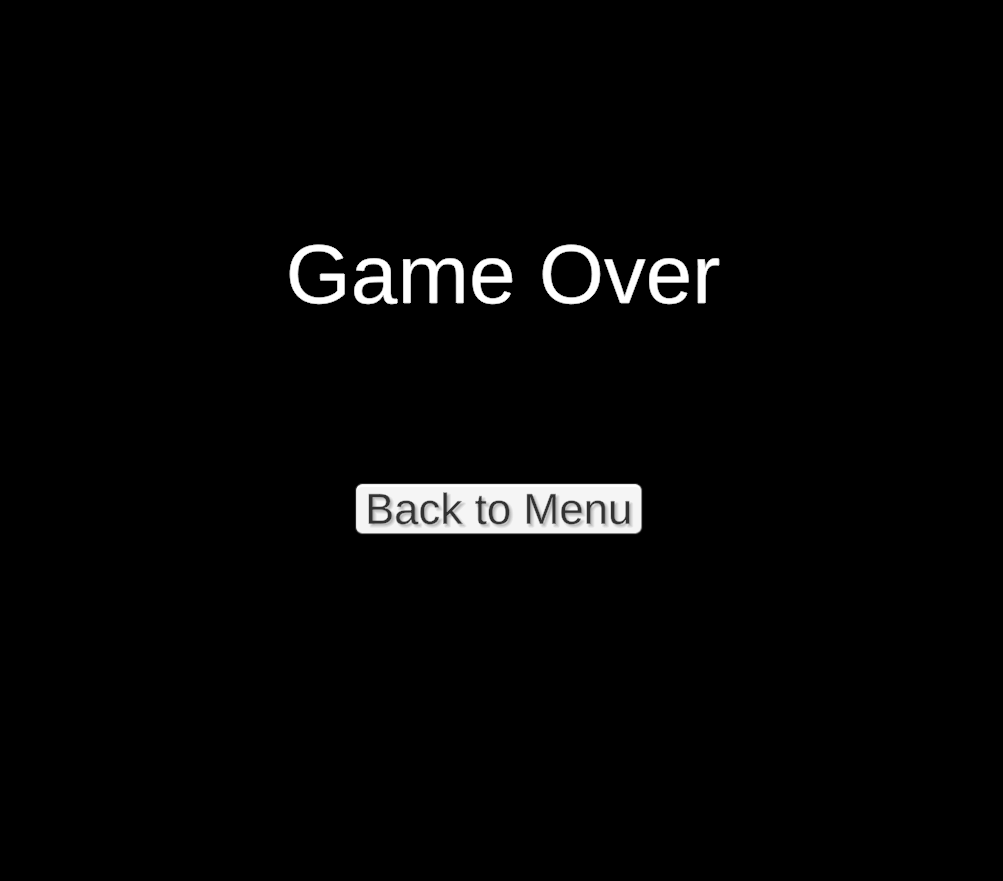
\includegraphics[width=\linewidth]{chapters/03/images/GameOver.png}
        \caption{Der Game Over Screen des Prototypen.}
        \label{UI02}
    \end{minipage}
\end{figure}



\section{Game UI und Spielmechanik-Anzeigen}

\begin{figure}[H]
    \centering
    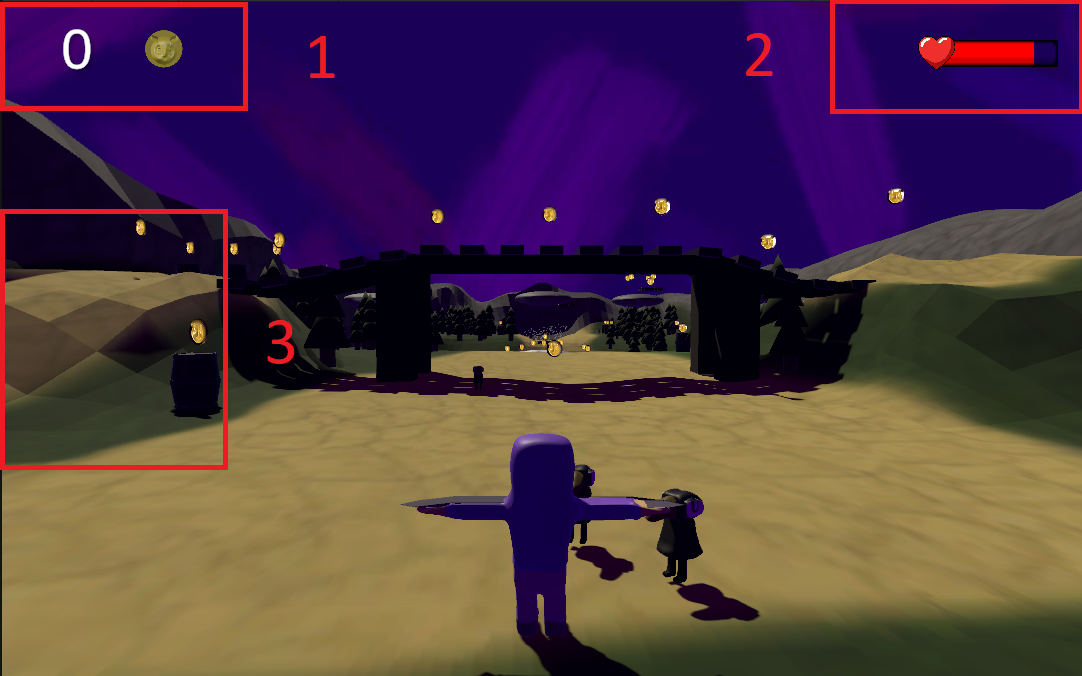
\includegraphics[width=0.8\textwidth]{chapters/03/images/GameUI.png}
    \caption{Das UI während des Spiels.}
    \label{htl03}
\end{figure}

\subsection{Eulenmünzen (1)}
Sammelobjekte, oder auch Collectibles gennant, gibt es in vielen Computerspielen. Jedoch bieten sie die unterschiedlichsten Funktionen. In PacMan ist das Sammeln von den Punkten teil des Spielziels. Verglichen zu Donkey Kong, wo das Sammeln von den Collectibles nicht verpflichtend ist. Aber es ist Teil von 101\% Vervollständigung des Spiels.
%https://donkeykong.fandom.com/wiki/Donkey_Kong_64#Gameplay

Als Sammelobjekt gibt es in dem Prototypen so gennante \glqq Eulenmünzen\grqq. Diese dienen ähnlich wie bei Donkey Kong als nicht verpflichtende Nebenaufgabe. Die Münzen schweben überall verstreut über die Welt des Prototypen. 

\subsection{Lebensanzeige (2)}

Eine Lebensanzeige in einem Computerspiel ist ein dezenter Hinweis darauf, dass der Spielcharakter sterblich ist. Schaden kann von Gegnern oder Fallen genommen werden.

In dem Prototypen wird die Lebensanzeige als roter Balken neben einem Herz dargestellt. Dieses Symbol befindet sich in der rechten oberen Ecke des Bildschirms. Lebensenergie wird abgezogen wenn die Spielfigur von einem Gegner getroffen wird oder in das \bettergls{void}{1} fällt.

\subsection{Steuerung (3)}
Die Idee war es die Steuerung auf dem User Interface darzustellen. Das ist ein einfacher Weg, das Spielkonzept dem Spieler näherzubringen. Ein gutes Beispiel dafür ist die Startwelt von Super Mario Odyssey. Dieses Spiel war auch eine große Inspiration für den Prototypen. 

\section{UI des zweiten Levels}
Das User Interface des zweiten Levels besteht aus einem Canvas mit UI Elementen und einer statischen Kamera von dem zweiten Level. 

In den nächsten zwei Listings wird erkenntlich gemacht, wie die Anzahl der Münzen zwischen den Scenen übergeben wird. Mithilfe des \verb+PlayerPrefs+ ist es möglich scenenübergreifend Werte in Variablen zu Speichern. 
% C#
\begin{lstlisting}[language=CSharp,caption={Portal Klasse.},label=code:portal]
    PlayerPrefs.SetString("HighScore", coinCounterText.text);
\end{lstlisting}

% C#
\begin{lstlisting}[language=CSharp,caption={GameManager Klasse.},label=code:gamemanager]
    Score = PlayerPrefs.GetString("HighScore");
    scoreText.text = Score;
\end{lstlisting}


\begin{figure}[h]
    \centering
    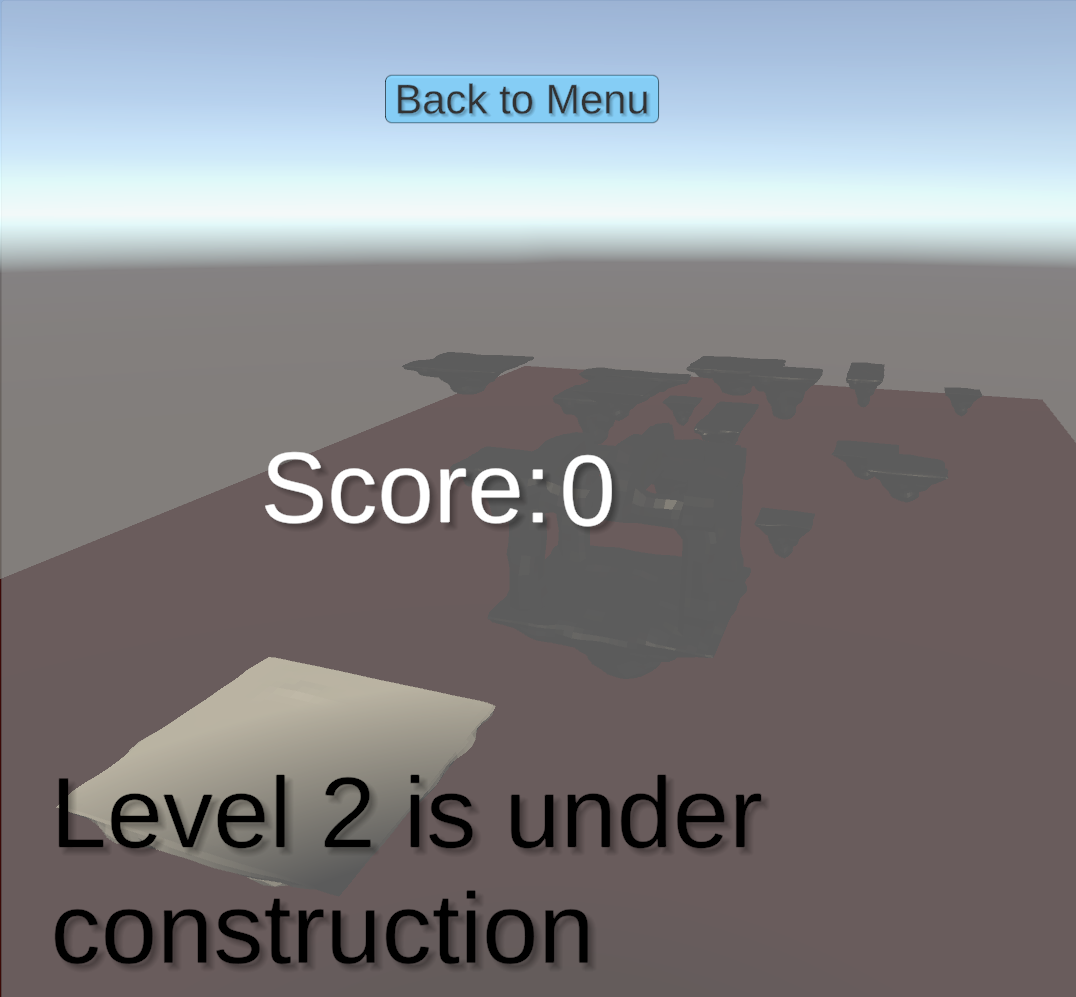
\includegraphics[width=0.6\textwidth]{chapters/04/images/V3/Level2Game.png}
    \caption{Der Endbildschirm des Prototypen.}
    \label{fig:UI20}
\end{figure}